\documentclass[12pt,a4paper]{article}
\usepackage{fontspec}
\setmainfont{Times New Roman}
\usepackage{indentfirst}
\usepackage{hyperref}
\usepackage{tikz}
\usepackage[left=2.64cm,right=2.54cm,top=2cm,bottom=2cm]{geometry}
\usepackage{geometry}
\usepackage{array}
\usepackage{color}
\usepackage{wallpaper}
\setcounter{page}{2}
\makeatletter
\definecolor{dkgreen}{rgb}{0,0.6,0}
\definecolor{gray}{rgb}{0.5,0.5,0.5}
\definecolor{mauve}{rgb}{0.58,0,0.82}
\usepackage{listings}
\pagenumbering{arabic}
\usepackage{fancyhdr}
\usepackage{lastpage}
\usepackage{minitoc}
\pagestyle{fancy}
\fancyhf{}
\rhead{21127158 - 21127511}
\lhead{HỆ THỐNG MÁY TÍNH}
\rfoot{Trang \thepage \hspace{1pt}/ \pageref{LastPage}}
\usepackage{multicol}
\setlength{\columnsep}{1cm}
\begin{document}
\thispagestyle{empty}
\begin{LARGE}
    \begin{center}{\underline{\color{red}{\bf NATIONAL UNIVERSITY OF HO CHI MINH CITY}}}
    \end{center}
\end{LARGE}
\vspace*{1cm}
\begin{center}{\Huge \color{blue}\textbf{PROJECT REPORT}}
\end{center}
\ThisCenterWallPaper{0.5}{fit.png}
\vspace*{15cm}
\begin{center}{\Huge \color{blue}\textbf{21CLC02 - Lê Hoàng Sang - 21127158}}
\end{center}
\begin{center}{\Huge \color{blue}\textbf{21CLC02 - Nguyễn Quốc Huy - 21127511}}
\end{center}
\vspace*{1cm}
\begin{center}
    {\Huge \color{blue}\textbf{{HỆ THỐNG MÁY TÍNH}}}
\end{center}
\newpage
\let\cleardoublepage\clearpage
\section{\textbf{\color{red}PHẦN 1: LỜI NÓI ĐẦU}}
\begin{itemize}
    \item \Large Đây là bài báo cáo về bài tập chuyển đổi cơ số Hệ Thống Máy Tính.
    \item \Large Yêu cầu chương trình chạy trên console.
    \item \Large Các thư viện cần thiết đã được nêu rõ trong chương trình.
    \item \Large Sinh viên thực hiện: Lê Hoàng Sang - 21127158
    \item \Large Sinh viên thực hiện: Nguyễn Quốc Huy - 21127511
    \item \Large Mã nguồn của 2 bạn được đồng bộ qua Github \\ \\
    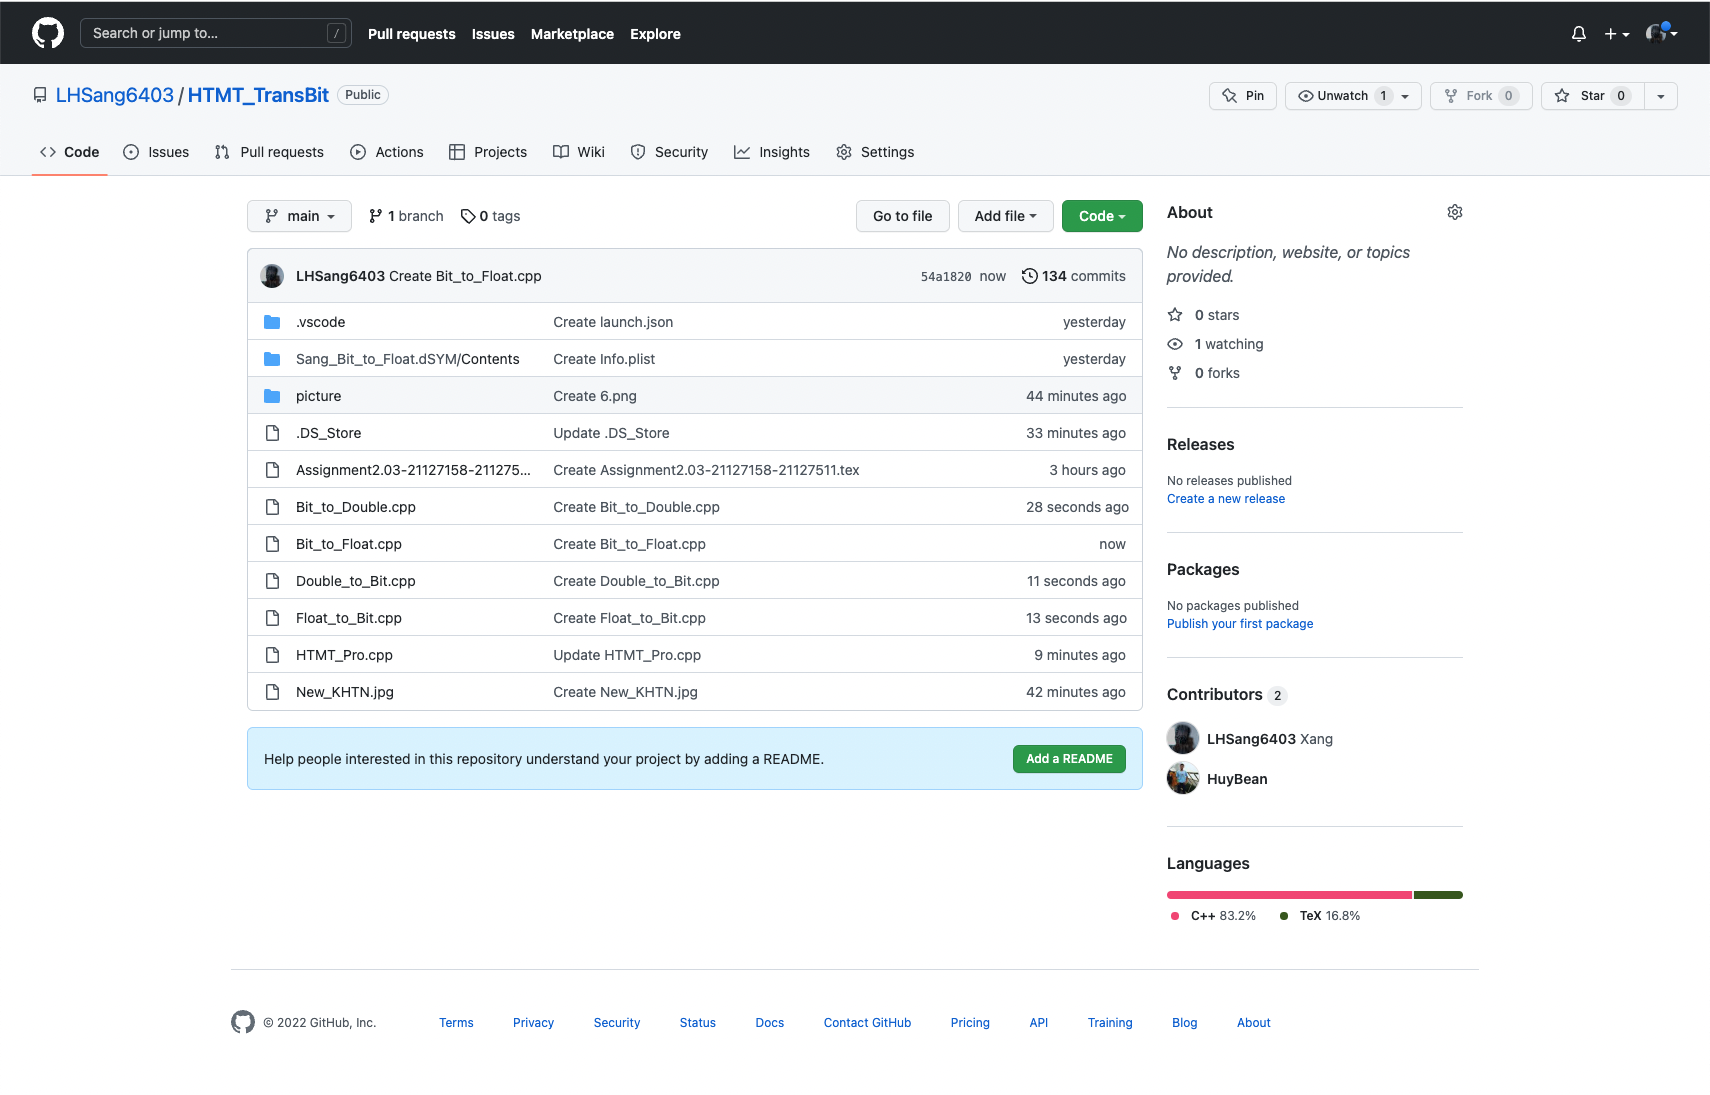
\includegraphics[scale= 0.2]{picture/Github.png} \\
    \item \Large Nguyễn Quốc Huy: Giao diện, báo cáo, các hàm chuyển đổi. \\
    \item \Large Lê Hoàng Sang: Báo cáo, các hàm chuyển đổi, Github. \\
\end{itemize}
\newpage
\tableofcontents
\newpage
\section{\textbf{\color{red}PHẦN 2: HƯỚNG DẪN}}
\large Hướng dẫn các thao tác trên chương trình:
\begin{itemize}
    \item  \Large Đầu tiên trên chương trình sẽ hiện Console mở đầu, người dùng cần \textbf{sử dụng phím mũi tên lên xuống hoặc phím 'w' hay 's'} để di chuyển đến lựa chọn của mình. \\
    \Large Sau đó nhấn dấu cách (spacebar) để xác nhận. \\
    \item  \Large Tiếp theo có các lựa chọn hiện ra như: Unsigned Char, Signed Short, Unsigned Int, Float,... đồng nghĩa với việc chuyển đổi dựa trên các kiểu dữ liệu tương ứng. \\
    \Large Người dùng cần trượt thanh trên màn hình console để thấy hết lựa chọn và thực hiện thao tác  \color{red}\textbf{CHỈ SỬ DỤNG PHÍM MŨI TÊN XUỐNG }\color{black} và nhấn spacebar để chọn. \\
    \item  \Large Sau mỗi kiểu dữ liệu đã chọn, trên màn hình sẽ tiếp tục hiện ra lựa chọn: \\
    \Large \textbf{Binary to Decimal}: Nhập dãy bit và cho chương trình chuyển về hệ thập phân. \\
    \Large \textbf{Decimal to Binary}: Nhập số ở hệ thập phân để chương trình chuyển về dạng bit. \\
    \item  \Large Sau đó, chỉ cần thực hiện phép nhập số cho chương trình theo yêu cầu đã chọn. \\
\end{itemize}
\newpage
\section{\textbf{\color{red}PHẦN 3: CÁC HÌNH MINH HỌA}}
\Large Sau đây là chi tiết các bước có được qua màn hình console. \\
\Large Đầu tiên, màn hình mở đầu của chương trình. \\
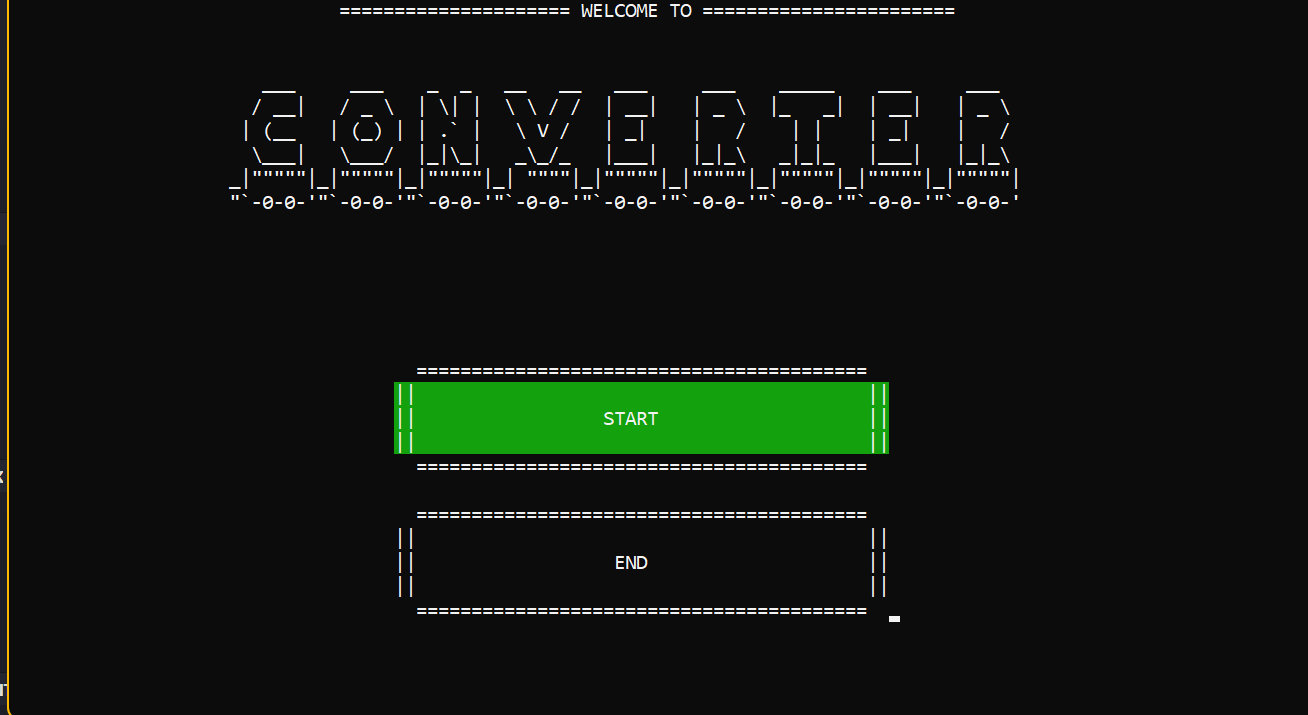
\includegraphics[scale=0.3]{picture/1.png} \\
\Large Kế đến là màn hình menu tùy chọn, người dùng cần trượt thanh trên console để thấy hết tùy chọn và thực hiện thao tác  \color{red}\textbf{CHỈ SỬ DỤNG PHÍM MŨI TÊN XUỐNG }\color{black} và nhấn spacebar để chọn.\\
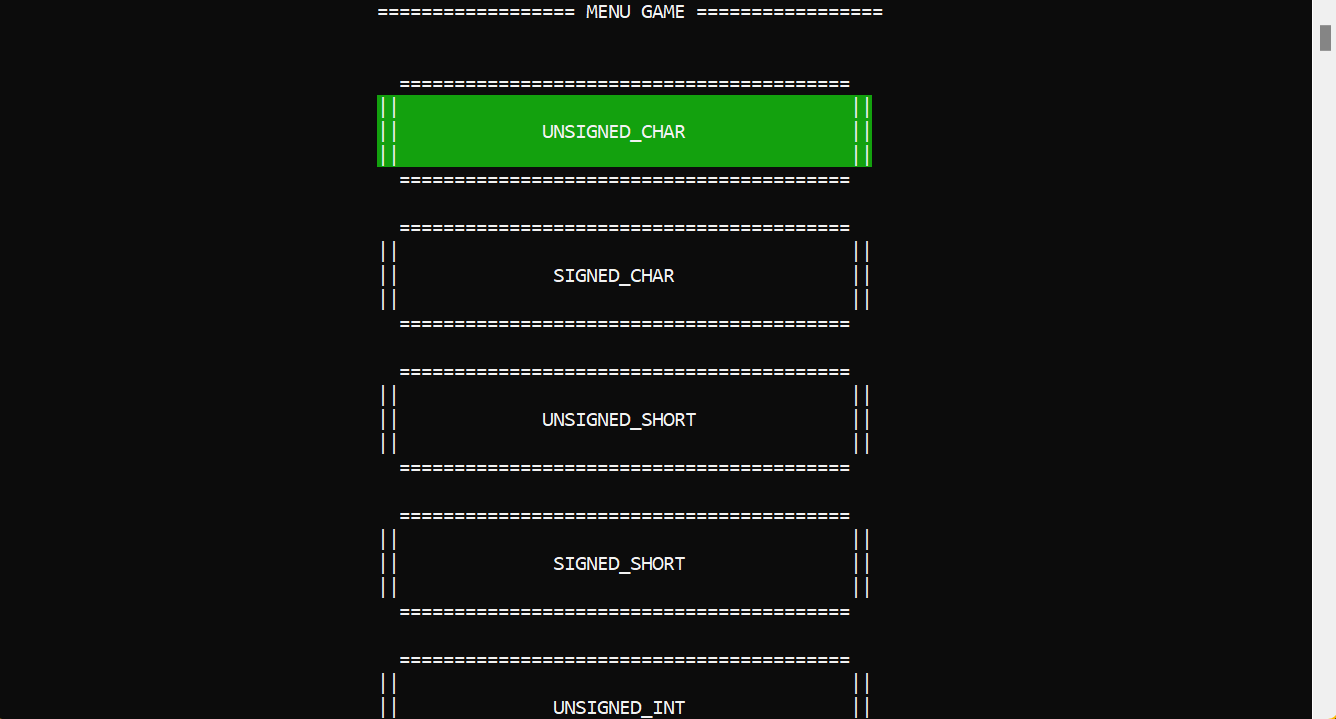
\includegraphics[scale=0.6]{picture/2.png} \\
\Large Tiếp theo là màn hình chọn chức năng chuyển đổi.\\
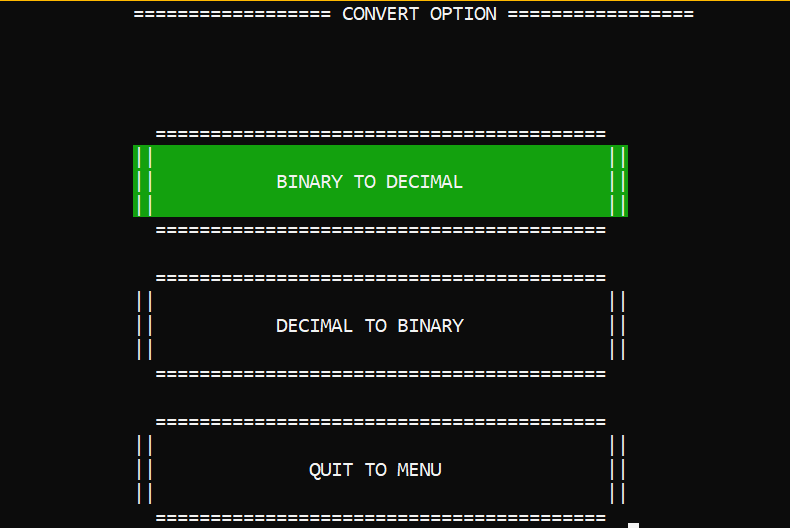
\includegraphics[scale=0.7]{picture/3.png} \\
\Large Đây là hình ảnh cho lựa chọn \textbf{BINARY TO DECIMAL}.\\
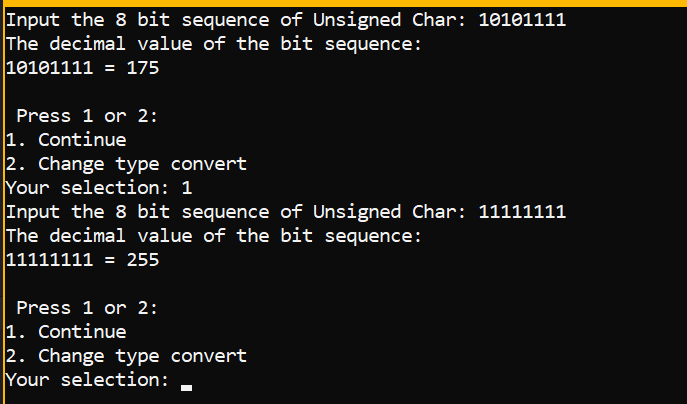
\includegraphics[scale=0.7]{picture/4.png} \\
\Large Và đây là hình ảnh cho lựa chọn \textbf{DECIMAL TO BINARY}. \\
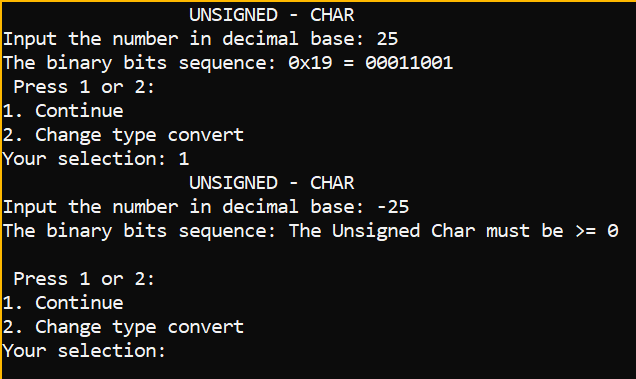
\includegraphics[scale=0.7]{picture/5.png} \\
\Large Còn đây là hình ảnh cho lựa chọn chuyển đổi \textbf{SỐ CHẤM ĐỘNG}. \\
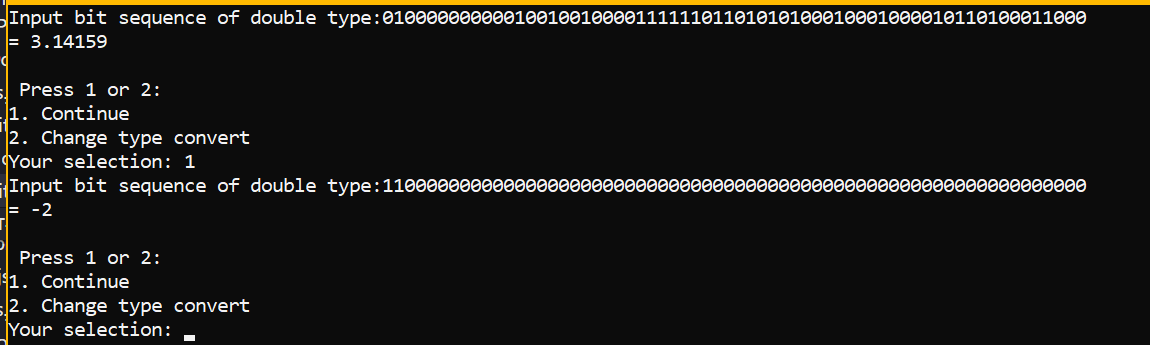
\includegraphics[scale=0.7]{picture/6.png} \\
\section{\textbf{\color{red}PHẦN 4: MÔ TẢ CÁC HÀM}}
\Large \subsection{\color{blue}\textbf{HÀM ĐÁNH DẤU} }
\begin{itemize}
    \item void $gotoxy$(short x, short y): Dùng để đưa các ký tự mong muốn đến tọa độ x y tương ứng trên console. \\
\end{itemize}
\Large \subsection{\color{blue}\textbf{HÀM CHUYỂN ĐỔI ĐƠN GIẢN} }
\begin{itemize}
    \item int $Convert$(char c): dùng để chuyển đổi các ký tự c nhập vào thành số nguyên trong trường hợp base > 10. \\
    Vd : $'A' = 10, 'B' = 11.... $
    \item double $toDeci$(char *str, int base): dùng để chuyển chuỗi nhập vào của một base cho trước ( 2 <= base <= 32) thành hệ cơ số 10.\\
    Chi tiết thuật toán:  \\
    Sử dụng hàm Convert bên trên để đổi từng ký tự thành số . \\
    Sau đó, tính tổng các phần tử sao cho mỗi phần tử sẽ nhân với số mũ mà sau mỗi lần cộng một phần tử vào, số mũ sẽ tăng lên base lần (số mũ lúc đầu = 1 do $base^0$ = 1). \\
    Quá trình tính sẽ được thực hiện từ phải sang trái. \\
    Vd :$ AAB_{16}$ = 11x1 + 10x16 + 10x16x16 = $2731_{d}$
\end{itemize}
\Large \subsection{\color{blue}\textbf{HÀM LÀM ĐẦY} }
\begin{itemize}
    \item void $fillbit$(long long x, int bit, int Signed): Dùng để bổ sung các ký tự còn thiếu trên dãy tương ứng vớt bit. \\
    Vd: $x = 111100, bit = 8, Signed = 1 \rightarrow  00111100$ \\
    Vd: $x = 101011, bit = 16, Singed = -1 \rightarrow 1111111111101011$ \\
    \item void $fillbitstring$(string str, int bit, int Signed): Tương tự như chức năng hàm trên nhưng áp dụng cho chuỗi string. \\
\end{itemize}
\Large \subsection{\color{blue}\textbf{HÀM CHUYỂN ĐỔI TỪ CHUỖI} }
\begin{itemize}
    \item string $findTwoscomplement$(string str): Dùng để chuyển chuỗi của một số âm(nếu có) sang bù 2.\\
    Chi tiết thuật toán: \\
    Tìm vị trí mà tại đó số 1 đầu tiên tính từ bên phải xuất hiện và đánh dấu.\\
    Thêm số 1 ở đầu chuỗi ( bit cực trái) \\
    Sau đó, tính từ vị trí số 1 đã đánh dấu, đảo ngược các bit phía sau: 1 = 0 và 0 = 1 cho đến khi gặp bit cực trái.\\
    \item string $ConvertFromDecimal$(long long from, int to): hàm này sử dụng đệ quy để đổi một số cho trước (from) từ base 10 sang base tùy chọn (to) và 2 <= base <= 32.  \\
    Chi tiết thuật toán: \\
    Tạo một biến tạm để lưu kết quả (res) sau mỗi vòng. \\
    Lấy số của hệ 10 chia lấy dư cho base và gán vào một biến (digit).\\
    Sau đó, đổi các số dư digit sang ký tự, nếu <10 thì đổi thành ký tự từ 1 đến 9 nếu >= 10 thì đổi thành A, B, C,… \\
    Tiếp theo gán ký tự vào biến kết quả để thành một chuỗi hoàn chỉnh. \\
    Sau mỗi vòng, số (from) sẽ giảm dần theo công thức: \\           
    from = from / base cho đến khi from = 0 ( đã xử lý xong) thì dừng hàm. \\
    \item string toBase16(unsigned num): chuyển một số nhập vào chuyển thành hệ 16 trong chuỗi.\\
\end{itemize}
\Large \subsection{\color{blue}\textbf{HÀM CHUYỂN TỪ DÃY BIT SANG SỐ} }
\begin{itemize}
    \item void $BitToDecimal$(int bit, int Signed): Yêu cầu người dùng nhập một số và chương trình sẽ chuyển về dạng nhị phân. Biến signed để xác định xem liệu kiểu dữ liệu đó là unsigned(không dấu) hay signed(có dấu).\\
\end{itemize}
\Large \subsection{\color{blue}\textbf{HÀM CHUYỂN TỪ CHUỖI BIT SANG DẠNG SỐ CHẤM ĐỘNG} }
\begin{itemize}
    \item void $format\_M$(char $*bin\_arr$, int $\&size)$: Dùng để rút gọn dãy bit, cụ thể ở đây là phần M(mantissa), nếu phía sau thừa số 0 thì có thể rút ngắn bớt.
    \item void $swap\_2Char$(char $\&a$, char $\&b$): Đảo vị trí 2 ký tự, đây là hàm bổ sung sẽ được áp dụng vào những hàm sau.
    \item char $*add0\_Fisrt$(char *M, int $\&M\_size$, int $p\_idx$, int $E\_val$, int $\&count\_multi$): trả về chuối có thêm các số 0 ở đầu chuỗi trong trường hợp E âm.
    \item void $multiply\_2Bin\_positive$(char *M, int $M\_size$, int $E\_val)$: nhân 2 chuỗi Bits trong trường hợp E dương.
    \item char $*multiply\_2Bin\_negative$(char *M, int $\&M\_size$, int $E\_val)$: nhân 2 chuỗi Bits trong trường hợp E âm.
    \item float $BinToNum\_f$(char *M, $int M\_size)$: chuyển từ Binary về dạng số, trường hợp Float.
    \item float $BinTo\_FloatPoint$(char *arr): xuất ra số Float hoàn chỉnh.
    \item double $BinToNum\_d$(char *M, int $M\_size)$: chuyển từ Binary về dạng số, trường hợp Double.
    \item double $BinTo\_DoublePoint$(char *arr): xuất ra số Double hoàn chỉnh.
\end{itemize}
\Large \subsection{\color{blue}\textbf{HÀM CHUYỂN TỪ DẠNG SỐ CHẤM ĐỘNG SANG CHUỖI BIT} }
\begin{itemize}
    \item int $countBit\_NeedMore\_f$(float input): trả về số Bits cần thêm.
    \item int $countBit\_NeedMore\_d$(float input): trả về số Bits cần thêm.
    \item long long $multiplyy$(float input): nhân số Bits cần thêm.
    \item char $*add\_pointBin$(long long input): thêm dấu chấm vào chuỗi Bits.
    \item int $count\_Exponent\_afterPoint$(char *res): đếm các Bits để tính E.
    \item int $count\_E\_value$(int exponent, int needMorebit): tính E.
    \item void $export\_bin\_f$(float input, char $*E\_arr$, char *man): xuất ra chuỗi Bits.
    \item void $export\_bin\_f$(float input, char $*E\_arr$, char *man): xuất ra chuỗi Bits.
\end{itemize}
\Large \subsection{\color{blue}\textbf{HÀM ĐỔI TỪ DECIMAL SANG BIT} }
\begin{itemize}
    \item void $Unsigned\_Char$(long long x): Dùng để kiểm tra tính hợp lệ của số nhập vào thỏa điều kiện Unsigned\_Char hay không, sau đó chương trình sẽ chuyển sang dạng nhị phân. \\
    \item void $Signed\_Char$(long long x): Dùng để kiểm tra tính hợp lệ của số nhập vào thỏa điều kiện Unsigned\_Char hay không, sau đó chương trình sẽ chuyển sang dạng nhị phân. \\
    \item void $Unsigned\_Short$(long long x): Dùng để kiểm tra tính hợp lệ của số nhập vào thỏa điều kiện Unsigned\_Short hay không, sau đó chương trình sẽ chuyển sang dạng nhị phân.\\
    \item void $Signed\_Short$(long long x): Dùng để kiểm tra tính hợp lệ của số nhập vào thỏa điều kiện Signed\_Short hay không, sau đó chương trình sẽ chuyển sang dạng nhị phân.\\
    \item void $Unsigned\_Int$(long long x): Dùng để kiểm tra tính hợp lệ của số nhập vào thỏa điều kiện Unsigned\_Int hay không, sau đó chương trình sẽ chuyển sang dạng nhị phân.\\
    \item void $Signed\_Int$(long long x): Dùng để kiểm tra tính hợp lệ của số nhập vào thỏa điều kiện Signed\_Int hay không, sau đó chương trình sẽ chuyển sang dạng nhị phân.\\
\end{itemize}
\Large \subsection{\color{blue}\textbf{HÀM MENU} }
\begin{itemize}
    \item void $INTRO$(int $\&key$): Dùng để tạo menu console mở đầu. \\
    \item void $INTRO\_NEXT$(int $\&key$): Dùng để tạo menu console cho các tùy chọn.\\
    \item $OPTION$(int $\&BinToDec$): Tạo menu hỏi rằng liệu người chơi nhập $Binary to Decimal$ hay $Decimal to Binary$.\\
    \item void $ConvertAgain$(int $\&Again$): Hỏi rằng người chơi có muốn tiếp tục convert hay đổi sang tùy chọn khác.\\
\end{itemize}
\section{\textbf{\color{red}PHẦN 5: TÀI LIỆU THAM KHẢO}}
\begin{itemize}
    \item \url{https://www.binaryconvert.com/convert_double.html} \\
    \item \url{https://en.wikipedia.org/wiki/Double-precision_floating-point_format} \\
    \item \url{https://en.wikipedia.org/wiki/Single-precision_floating-point_format} \\
    \item \url{https://www.google.com/search?q=float+to+bit&sxsrf=ALiCzsbDJ8EnsSrW7UlVZsBpkWm3qBS5Rw%3A1654418958742&ei=Dm6cYvn4LP-MseMPyMyAkAw&ved=0ahUKEwj5t-Hy9pX4AhV_RmwGHUgmAMIQ4dUDCA4&uact=5&oq=float+to+bit&gs_lcp=Cgdnd3Mtd2l6EAMyBggAEB4QBzIFCAAQywEyBQgAEMsBMgUIABDLATIICAAQHhAIEAcyCAgAEB4QCBAHMgoIABAeEAgQBxAKMggIABAeEAgQBzIICAAQHhAIEAcyCAgAEB4QCBAHOgcIABBHELADOgQIABAeOgYIABAeEAU6BwgjELACECc6CAgAEB4QBxATOgQIABATOgoIABAeEAcQBRATOgwIABAeEAcQBRAKEBM6CggAEB4QCBAHEBM6BQgAEIAEOggIABAeEAcQCjoICAAQHhAPEAdKBAhBGABKBAhGGABQmwNY4hxgwCFoA3AAeACAAa0BiAGGDpIBBDEuMTSYAQCgAQHIAQjAAQE&sclient=gws-wiz} \\
\end{itemize}
\begin{center}
\LARGE \textbf\underline{{HẾT}}
\end{center}
\end{document}